\documentclass[../main.tex]{subfiles}

\graphicspath{{../images/}}

\begin{document}
\pagestyle{fancy}
\chead{Module 3}
\rhead{Junseo Shin}
\lhead{CSE 4059}

% reset figure numbering to Fig 1, Fig 2, 3, ... without section number
\renewcommand{\thefigure}{\arabic{figure}}

\section*{Vector Add}

\begin{figure}
    [ht]
    \centering
    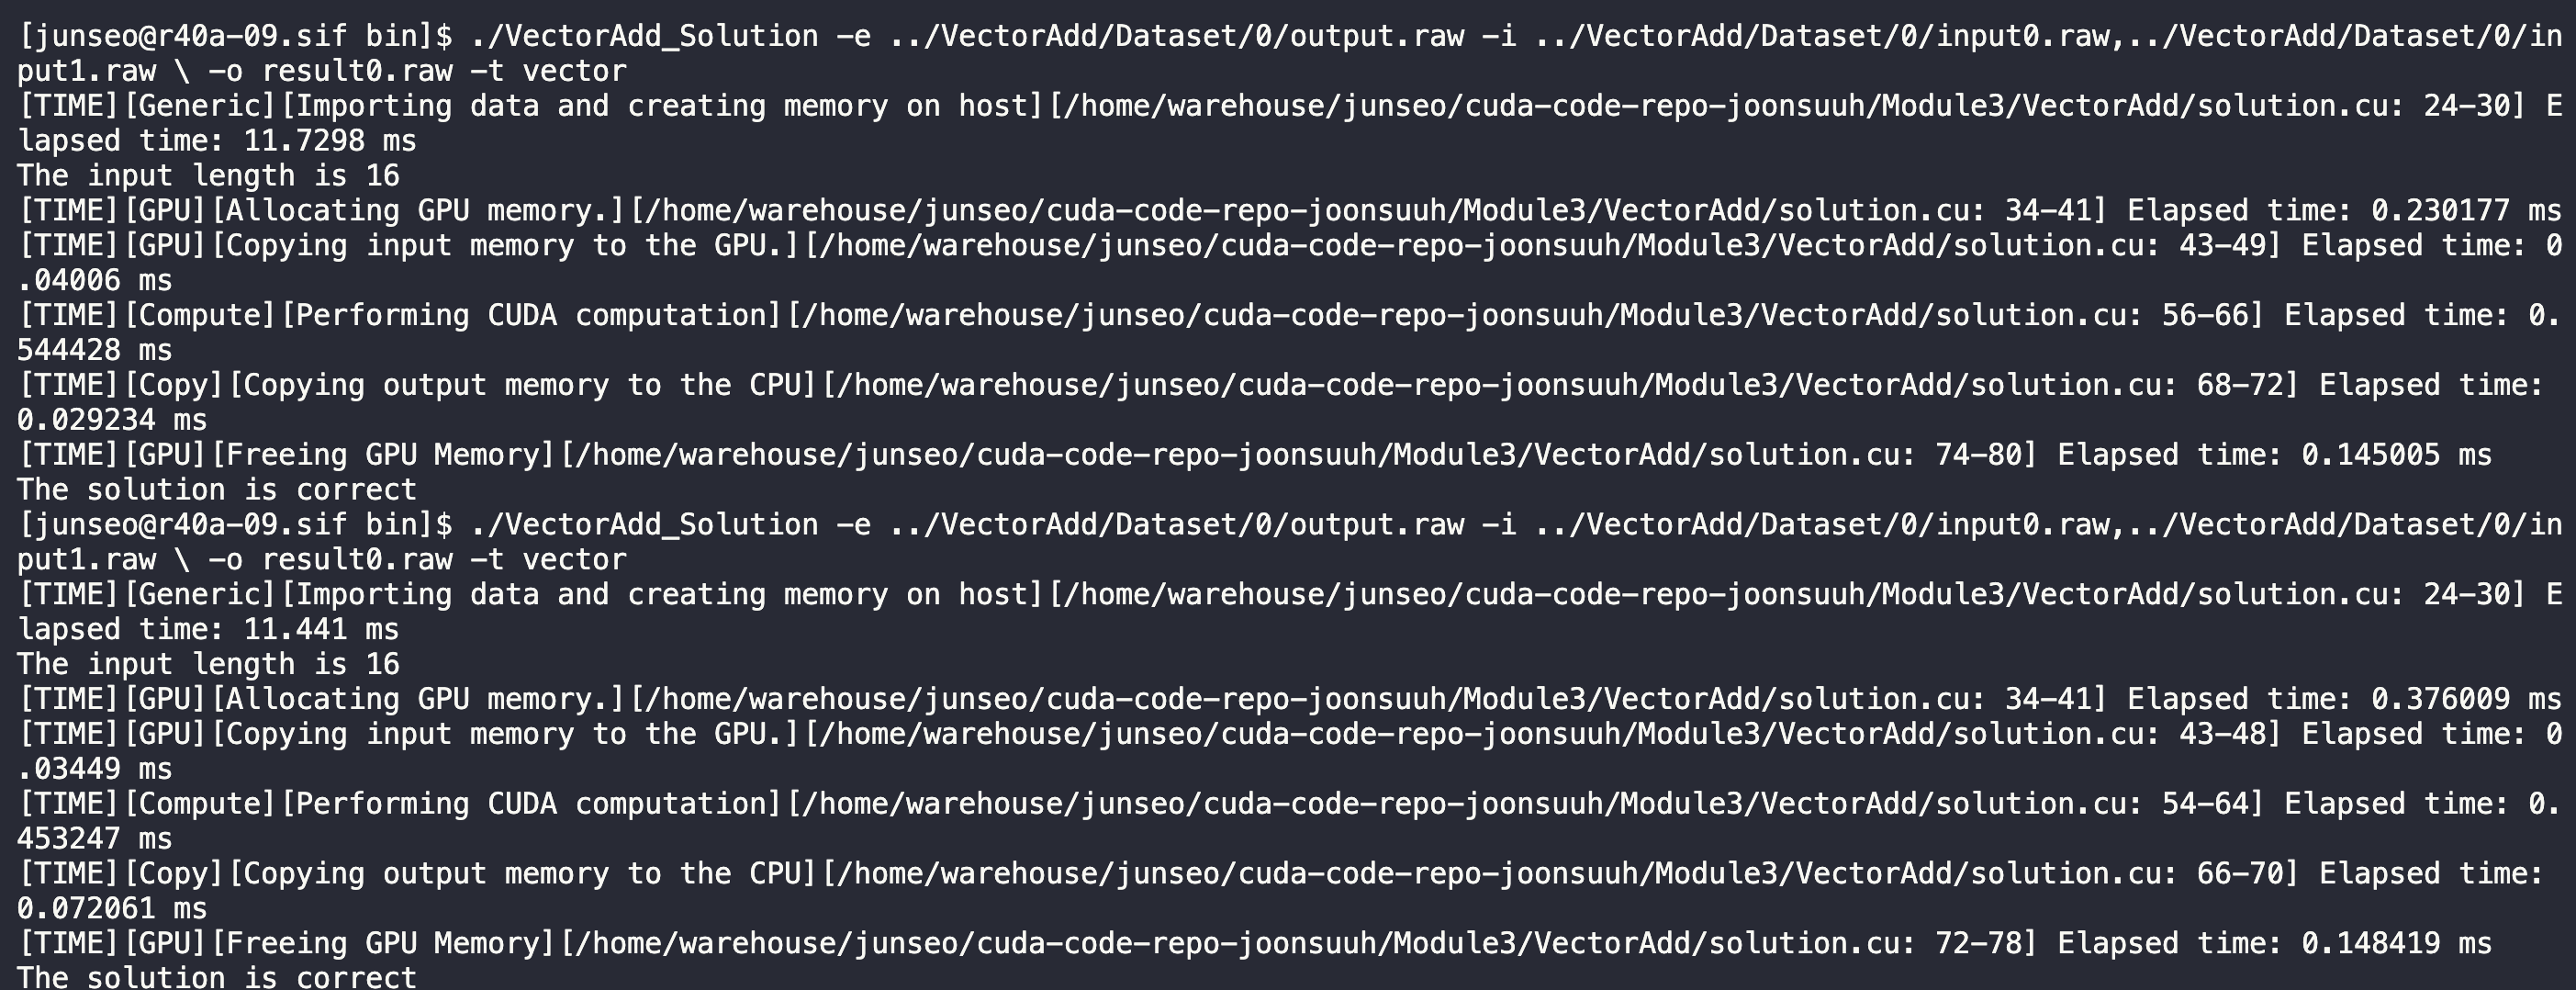
\includegraphics[width=0.8\textwidth]{vectoradd.png}
    \caption{\texttt{VectorAdd\_Solution} output}
\end{figure}

\subsection*{Questions}

\begin{enumerate}
    \item How many floating operations are being performed in your vector add
    kernel? EXPLAIN.

    The kernel perfroms \texttt{inputLength} floating point operations. This is because
    the if statement in the kernel function \texttt{index < len} limits the number of threads that
    are actually performing the floating point operations.

    \item How many global memory reads are being performed by your kernel?
    EXPLAIN.

    The kernel performs \texttt{inputLength * 2} global memory reads because each thread
    reads an element each from the two input arrays.
    
    \item How many global memory writes are being performed by your kernel?
    EXPLAIN.
    
    The kernel performs \texttt{inputLength} global memory writes because each thread writes 
    to the output arrary in the if statement.

    \item Describe what possible optimizations can be implemented to your kernel
    to achieve a performance speedup.

    We can achieve a performance speedup by using block sizes that are a multiple of the warp size
    (32) and using shared memory to reduce the number of global memory reads and writes.
    
    \item Name three applications of vector addition.
    
    \begin{enumerate}
        \item [i] Image processing (e.g. blur, translating an image on a screen)
        \item [ii] Phyics simulations (e.g. N-body simulations require vector addition to find the net
            force and momenta of N-particles)
        \item [iii] Single value decomposition (SVD) (e.g. crude image compression
        \href{https://timbaumann.info/svd-image-compression-demo/}{[web demo]} uses SVD which
        requires matrix multiplication and vector addition)
    \end{enumerate}
\end{enumerate}



\end{document}